\lettrine{I}{n} this chapter, you describe all of the things that the reader would need to know in
order to understand the rest of the thesis. Save anything that is unique to your work
for Chapter 3. Chapter 2 should only include information that is general in nature.
For example, if you are designing a new routing protocol, you would describe routing
protocols in general in Chapter 2, and leave your actual protocol design for Chapter 3.
One of the main purposes for Chapter 2 is to make it easier to write Chapter 3,
because when you get to the various topics already covered in Chapter 2, you can just
reference back to that chapter, rather than have to describe the basic theory along with
whatever you uniquely did.

\section{Introduction}
\lettrine{T}{his} chapter provides an introduction to... Section \ref{sec:routing} describes how Internet Protocol (IP) routing works generally and Section \ref{sec:hopping} discusses IP address space randomization. Section \ref{sec:ipv6} discusses details of IPv6 packets, including how Extension Headers work. Section \ref{sec:ipsec} covers IPsec. % needed?
Section \ref{sec:totp} provides a description of Time-Based One Time Pads (TOTP). Finally, Section \ref{sec:related_research} examines previous effects in IP address hopping.

\section{Internet Protocol}
\par This thesis makes the assumption that the reader has a famility with how Internet Protocol (IP) works. However, several aspects of this protocol are critical to the functioning of the system described later and are detailed here. 

\subsection{IP Routing}
\label{sec:routing}
\par IP packets are routed from system to system based on the destination address contained in their header. IP version 4 uses 32-bit addresses to uniquely identify each system on the public Internet. These addresses are typically represented in a ``dotted quad'' format: for example, 74.125.228.36. IP version 6 uses 128-bit address, typically represented in heximdecimal separated by colons (i.e. \texttt{a3d3:2d42::8c24}).

\par Regardless of which version is in use, high-level routing remains the same. When a router receives a packet, it examines its routing table and decides what interface to send the packet out on based on the most specific entry in the table. This scheme allows a router to direct packets without having to know every individual IP, they only have to know broad swaths of addresses. A corporation's network, for instance, may contain hundreds or thousands of addresses, but the routers directing packets to them need only have one entry in their table to correctly route packets to them. The internal routers of the corporation are then in charge, a key fact that allows IP hopping to work.

\subsection{IPv6 Packet Structure}
\label{sec:ipv6}
\par IPv6 and IPv4 packets are rather different with packet structure, with IPv6 eliminating much of the cruft and complication in the older standard. This was done by eliminating packet fragmenting, checksums at the network layer, 

\section{IP Hopping in Detail}
\par Address hopping is a simple concept at a high level: take the basic identifiers of a network and mutate them in a way that only those we wish to communicate with can follow. Doing so makes it difficult for an adversary to correlate sniffed traffic with individual machines and even more difficult to probe into the network to enumerate hosts. In trying to actually implement such a system, however, several issues arise. 

\par To aid the discussion of these problems we will use the example network illustrated in Figure \ref{fig:exnetwork}. As it shows, we have two main networks \textit{A} and \textit{B} that are assigned the displayed IP ranges, are connected by the Internet, and have an interest in communicating freely with one-another. Each of these has a few friendly ends nodes (\textit{A1}, \textit{A2}, etc) behind a main router (\textit{AR} and \textit{BR}). Additionally, network \textit{B} has a potentially rogue client inside it named \textit{M1}. Outside of those two networks, we see the friendly \textit{C2} node, who has an interest in at least occasionally communicating with nodes inside \textit{A}/\textit{B}, and malicious \textit{M2}, who wants access to said networks. The details of the routes between them and \textit{A} and \textit{B} are inconsequential.

\par Note that for the sake of this discussion non-routable IPv4 addresses are largely used. This is done merely for convenience and readability, the discussions apply to IPv6 as well unless otherwise noted.

\begin{figure}
	\centering
	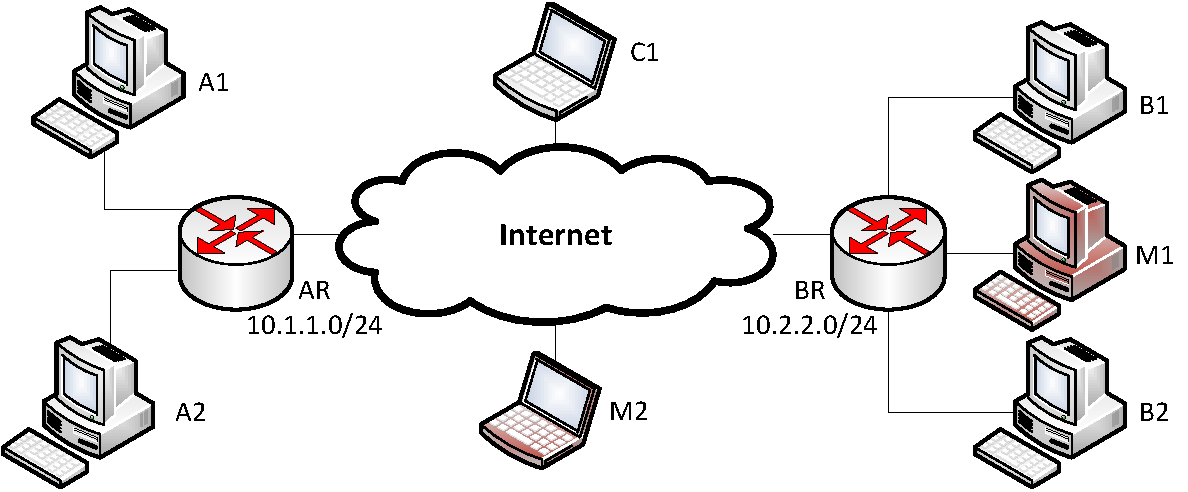
\includegraphics[width=0.75\textwidth]{../diagrams/exnetwork}
	\caption{Example network layout \tbd{include IP addresses}}
	\label{fig:exnetwork}
\end{figure}

\par There are two basic ways IP address hopping could be deployed on this network: each end point hops individually or the network gateways transform incoming and outgoing packets. Both options and their strengths and weaknesses are discussed below.

\subsection{End Point Hopping}
\par For the example network, each end point hopping would mean that all of the nodes behind \textit{AR} and \textit{BR} (\textit{A1}, \textit{A2}, \textit{B1}, etc.) change addresses on a periodic basis, independent of one another. Despite the apparent simplicity of this setup, several questions must be answered.

\par First, how do the nodes keep track of one another? If every node knows about all the others, then scalability might become an issue, as every client presumably has to maintain some amount of data on fellow hopping clients to determine where each one is at any given time. It may be possible to devise a scheme where this flaw is mitigated by having all clients hop using the same secret and they each know just the broad IP ranges where fellow hoppers reside (i.e., the \textit{AR} nodes know that 10.2.2.0/24 is a network they talk to with hopping), but this accentuates the next question: how do clients choose their hops?

\par Clearly, each node must know some secret from which IP addresses are generated, hopefully in a manner which appears random to outsiders yet is predictable for those with the secret (the ``hopping pattern''). There may be only one of these secrets, which every node in the protected network knows---that is, the nodes in both A and B, hereafter collectively referred to as the ``hopping network.'' This does have the potential flaw of revealing too much information to an eavesdropper though: with a large number of nodes all following a hopping pattern based on the same key, it may be easier to deduce the secret. If one assumes that end-point hopping would \textit{have} to employ a single key to remain scalable, then the first flaw in this setup becomes obvious.

\par Just as importantly, however, is the question of how nodes coordinate their IP address choices. IP routing requires addresses follow a largely hierarchical setup, with broad ranges like 10.0.0.0 leading to 10.1.0.0 to 10.1.1.0 and so on. Thus, if \textit{A} has the network address range 10.1.1.0/24, then all of its nodes should fall within the address range of 10.1.1.1 through 10.1.1.255. This means that when each node hops it must remain within the valid range of the network it is a part of \textit{and} that the address it chooses must not already be taken another node. Given enough nodes in a subnet, a conflict is quite possible, leading to unpredictable network behavior. 

%\par It is likely possible to devise a reasonably robust algorithm for all nodes to hop simultaneously and end up on unique IPs, but this encounters a few issues with the link-layer of a network's architecture. On local networks, machines are identified by a Media Access Code (MAC) and systems must map IP addresses to the hardware MAC using Address Routing Protocol (ARP). Nodes virtually always cache this information for speed, so for the period of time from a hop to the cache entry expiration time, packets sent to nodes on the local network will likely contain an incorrect MAC and not arrive at the correct destination. TCP would then detect the packet loss and retransmit, trying until either the connection timed out or the ARP cache updated. Even if ARP information is only cached for a few seconds, at best this could result in bursts of traffic on local networks and at worst dropped connections. A similar problem also exists at the switches in the network, although this would likely resolve itself quickly.

%\par It would be possible to work around this issue by having whatever utility is handling the hopping also alter the ARP cache. To do so, every node would need to compute the correct locations of all other nodes and do so at precisely the same time. While not infeasible, this becomes even more platform-specific than the general IP hopping was. Approaching it the other way, nodes could all send gratuitous ARPs when their IP changes, but this still generates extra traffic on the network and \textit{forces} systems to be extremely vulnerable to ARP spoofing, a common part of a network attack.

\par The easiest solution to this problem is to give each node a unique, non-overlapping address range in which to hop. This avoids the ARP problem because there will never be a different node that used to have the same IP but a different MAC. However, this has the difficulty of requiring a large enough address space to make hopping beneficial. If a given node only has five possible addresses in which to hop, for instance, it becomes trivial for an attacker to just keep trying a single one until the node returns to it. IPv6 would avoid this problem, as the Internet Engineering Task Force recommends the allocation of a /64 address space ($2^{64}$ addresses) to every link \cite{rfc3267}, but IPv4 with its extremely limited address space would not allow this flexibility and, unfortunately, the reality of current networks mandates support for IPv4. \tbd{TBD see if a paper has an analysis of the needed address space for usability}

\par Despite these negatives end point hopping does have advantages. First, scalability issues lie more in storage space and key lookup than actual computation, as every node only has to perform packet transformations for their own ingress and egress packets. Although not discussed yet, it is likely that any IP hopping scheme will also incorporate packet encryption, so distributing this load certainly cannot hurt. Second, end point hopping protects clients from probing no matter where the adversary is in the network. For example, as long as \textit{M1} in our example network lacks the hopping key, they have no more of an advantage in scanning any of the \textit{A} or \textit{B} nodes than \textit{M2}, who is outside the network. Finally, end point hopping comes with the ability for individual nodes such as \textit{C1} to connect to the main hopping network, without requiring any additional work or software development.

\subsection{Gateway hopping}
\par The alternative to end point hopping is to move the hopping to network gateways. In such a scheme, networks are placed behind gateways that alter all traffic passing through them appropriately. What ``appropriately'' means varies with every implementation, but in one way or another, a gateway outside of the actual end points alters the IP traffic to make it appear as though the systems inside are changing IP addresses.

\par Nodes inside the network may or may not have knowledge of the hopping. In most instances the hopping occurs with no modification of the end points and is largely transparent. This need to only deploy a small number of systems, rather than altering every system, gives gateway-based hopping an advantage over end point-based on larger networks. Applying software and/or hardware changes to every system is costly in terms of both time and manpower. Even more significantly, legacy systems running older operating systems would likely need custom solutions and might be completely unsupportable as a result.

\par The most common observable side effect of gateway hopping (beyond the latency associated with the additional processing) is TCP connection dropping. Because TCP depends on IP addresses and ports numbers to identify on-going connections, any alterations to this information would traditionally kill the connection. This is a problem also faced by end point hopping schemes, but is more easily corrected because the individual machines know the state of connections and can correct appropriately. With gateway hopping, however, the situation can be much more delicate and likely requires significant state tracking at the gateway.

\par Because of this required state tracking and the need for a single system to alter all traffic in and out of an entire network, gateway-based hopping presents a possible performance problem. This should not be an insurmountable obstacle, however, and some studies have already shown a CPU impact of around 10\% \cite{TAO} (even when encryption was being applied). Additionally, gateway hopping has difficulty with individual nodes connecting to the network. In \textit{C1}'s case, for instance, it would likely need software for just the individual machine, almost exactly as an end-point hopping scheme would require.

\section{IPsec}
\label{sec:ipsec}
\par IPsec is a common standard for establishing encrypted and/or authenticated connections. Rather than working at the transport and session layers---i.e., SSL in conjunction with TCP---, IPsec functions on the network layer. \tbd{cite IPsec rfc, layer info}  

\section{Time-Based One Time Pad}
\label{sec:totp}
\tbd{TOTP description, how to get more than the default number of bits}

\section{Previous Implementations}
\label{sec:related_research}
\par With the proceeding discussion in mind, let us look at some previous implementations of this concept and the important results from their experimentation.

\subsubsection{BBN's Dynamic Network Address Translation (DYNAT)}
\par In 2001, BBN Technologies released a paper entitled ``Dynamic Approaches to Thwart Adversary Intelligence Gathering'' \cite{BBNDYNAT}. In this paper, they set out to test the hypothesis that ``dynamic modification of defense structure improves system assurance.''

\par Their dynamic network address translation (DYNAT) technique, as they called it, was put through a series of red-team experiments to test if it decreased an adversary's ability to map the network. The experimentation confirmed BBN's hypothesis: DYNAT did in fact increase system assurance because the adversary's work greatly increased compared to static networks. Even when the red team was given intimate knowledge of DYNAT's operation, the adversary could not identify a critical server in an enclave with DYNAT active.

\par The BBN's DYNAT implementation focused on individual clients connecting to a server enclave, through a DYNAT gateway on the server end. This gateway transformed incoming and outgoing packets between ``true'' host identification information---e.g., the actual IP address and port number of a server inside the enclave's network---and values which varied based on a pre-shared key and time. On the client side, a ``DYNAT shim'' sat in the network stack and did the same thing, transparently allowing client applications to work with the server enclave. Additionally, DYNAT applied encryption to all traffic for confidentiality.

\par BBN's experiments also demonstrated that the encryption of the packets was critical, as the attackers could trivially sniff the traffic to find important servers, even if they did not know the real IP address or port of the target. For example, an attacker could see a packet contained a HTTP response and thus learn an active IP and port for a web server, even if probing for it was impossible. While this information would only be valid for a limited period, it may be enough time for the attacker to compromise the internal network.

\subsubsection{Sandia Dynat}
\par In 2002, Sandia National Labs released a final report on their extensive work in the ``dynat'' field \cite{SandiaDynat}, as they refer to it. This report covers virtually every variable in a dynat system, from how hopping is synchronized to where in the network it is implemented. This paper points to many of the important issues that must be considered when implementing or deploying a dynat.

\par Of particular importance to our implementation proposal (ARG) are Sandia's recommendations on the location of the deployment of a gateway-based dynat. In order to avoid interference with existing firewall rules---particularly ones with a stateful firewall---, a dynat must be deployed beyond the current system. Likewise, for gateway-based virtual private networks (VPN), there is often a static IP requirement to allow for authentication \cite{SandiaDynat}, so a IP hopping gateway must also lie beyond the VPN concentrator. Essentially, the hopping gateway should be the last system before each the network connects to the outside world \cite{SandiaDynat}.

\par The Sandia report also provides significant insight into the interaction of a dynat with IPSec and strongly suggests a combination of the two. First, the encryption from IPSec avoids the ineffectiveness of dynat if the packets can be trivially sniffed for information, as already discussed in \cite{BBNDYNAT}. Second, IPSec is strengthened with the addition of a dynat, as the dynat can quickly reject invalid packets based on invalid source and destination identifiers, rather than forcing IPSec to perform expensive HMAC computations and/or encryption. However, the report also warns that the use of IPSec with dynat can reduce some aspects of dynat's access control because more identifiers are encrypted and unusable.

\subsubsection{Applications Participating in their Own Defense (APOD)}
\par In 2003, BBN proposed another IP hopping implementation as part of the Defense Advanced Research Projects Agency (DARPA) Applications that Participate in their Own Defense (APOD) project \cite{APOD}. This system was a refined version of the previous BBN DYNAT, featuring a network address translation (NAT) gateway sitting either on the server host itself or on a gateway into the network.

\par As noted by the authors, the primary differences between APOD and the previous DYNAT related to implementation. Whereas the BBN DYNAT was a very specialized solution, APOD employed standard Commercial Off The Shelf (COTS) utilities, such as Linux's iptables, to perform much of its work. They furthermore noted that APOD could be implemented as a NAT gateway on the networks of both the client and the server, the approach chosen for ARG.

\subsubsection{Network Address Space Randomization (NASR)}
\par The 2005 Network Address Space Randomization (NASR) was an IP address hopping system designed to defeat hitlist-based worms \cite{NASR}. These worms spread to pre-collected lists of IP addresses and typically propagate much faster than traditional worms that target random IPs. To fight this, NASR caused the pre-built hitlists to decay by changing IP addresses on a periodic basis.

\par The most unique aspect of this research was the use of Dynamic Host Configuration Protocol (DHCP) to force the changes. Through the use of a slightly intelligent DHCP server that leased IPs for a only a short time frame (on the order of tens of minutes) and only offered IPs that have not been used recently, most networks already using DHCP can be quickly changed to a randomized scheme. This simplicity does come at a cost, however: TCP connections are killed whenever the IP change occurs, forcing the hopping period to be quite long or risk unacceptable connection losses. The researchers did introduce intelligence into the DHCP server to allow it to detect ``long-lived'' TCP connections (i.e., a download) and give clients the same IP if they appeared busy. Beyond that, they also monitored what services a client was using, as many are resilient to a connection being torn down \cite{NASR}.

\par Despite those improvements, address changes occurred even in the fastest of instances only once an hour or so. This met the goal of hitlist worm protection, but is likely inadequate for obfuscating the network from a more intelligent enemy.

\subsubsection{Network Address Hopping (NAH)}
\par In 2005, European researchers presented a system they named Network Address Hopping (NAH) \cite{NAH}. This system focused on a client contacting a server as a negotiable protection measure, rather than an always-on system used between pre-configured systems.

\par A protocol employing IPv6 allowed a client to tell a server that they supported (and wished to use) NAH. If the server supported NAH, it replied with its hopping pattern. The client then sent its own hopping pattern, before reconnecting using the pattern the server just gave it. Packet count per connection was used to synchronize the hops and detect lost packets.

\par Once again, the NAH authors noted that encryption was important to maintaining the confidentiality of the data stream. However, they also stated that without encryption the system still provided some benefit, as packets bound for ``different'' addresses might follow differing routes due to the different (perceived) destinations. This means an attacker would need to either compromise a route fairly close to an endpoint to ensure they saw all traffic or compromise every possible route and collate the traffic together. Even if they manage to accomplish that, the attacker would still have to collect all traffic passing them in order to reconstruct the full stream (because they are unable to filter for specific IPs to identify the connection they are interested in), which poses a storage and computation problem given enough data \cite{NAH}.

\par As an additional side effect of the variable routing, the researchers noted that such a system may actually increase the throughput and reliability of a system. If multiple routing paths are used, congestion may be avoided and traffic ultimately flows more smoothly \cite{MultimediaDistributed}. While this is not viewed as an important aspect of this system, the potential does add support to the employment of address hopping.

\subsubsection{Transparent Address Obfuscation}
\par Finally, in 2006 a system called Transparent Address Obfuscation (TAO) was proposed \cite{TAO}. This system focused on protection of the Internet as a whole from hitlist-based worms and was somewhat based on the previous work in NASR \cite{NASR}. It featured gateways on networks that maintained external-to-internal address mappings for all nodes inside the protected network, with the external addresses changing with a configurable frequency. To maintain existing connection regardless of mapping changes, TAO included a NAT table. 

\par A disadvantage of this design was address space overhead. Testing showed that around 10\% more address space was needed for three simulations on large-scale networks, based on the need to reserve addresses to maintain connections while continuing to change address mappings. However, TAO had the distinct advantage of only requiring the addition of a single box at the network's edge and no cooperation from remote hosts was needed for it to provide its services.
